\begin{figure}
	\centering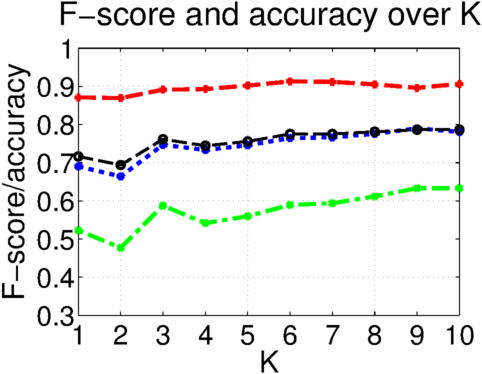
\includegraphics[width=0.3\textwidth]{tex/appendices/test/zcr11FP.png}
	\centering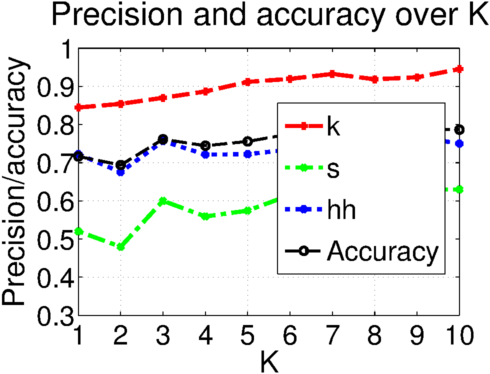
\includegraphics[width=0.3\textwidth]{tex/appendices/test/zcr11_P.png}
	\centering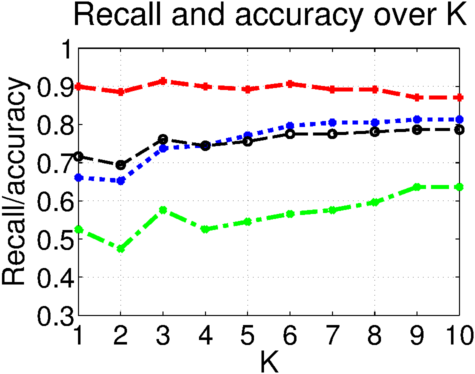
\includegraphics[width=0.3\textwidth]{tex/appendices/test/zcr11_R.png}
	\caption{Plots over K for Zero Crossing Rate}
\end{figure}


\begin{table}
\begin{subtable}[tbp]{0.45\textwidth}
\centering
\begin{tabular}{|c|c|c|c"c|}
\cline{2-5}
 \multicolumn{1}{c|}{} & \textbf{k}  & \textbf{s}  & \textbf{hh}  & Prec.\\ \hline
 \textbf{s} & \textcolor{red}{0.899} & 0.172 & 0.051 & 0.845\\ \hline
 \textbf{k} & 0.101 & \textcolor{red}{0.525} & 0.288 & 0.520\\ \hline
 \textbf{hh} & 0.101 & 0.303 & \textcolor{red}{0.661} & 0.722\\ \Xhline{2\arrayrulewidth}
 F & 0.871 & 0.523 & 0.690 & \textcolor{blue}{0.716}\\ \hline
\end{tabular}
\caption{$K=1$}
\end{subtable}
\hfill
\begin{subtable}[tbp]{0.45\textwidth}
\centering
\begin{tabular}{|c|c|c|c"c|}
\cline{2-5}
 \multicolumn{1}{c|}{} & \textbf{k}  & \textbf{s}  & \textbf{hh}  & Prec.\\ \hline
 \textbf{s} & \textcolor{red}{0.885} & 0.162 & 0.042 & 0.854\\ \hline
 \textbf{k} & 0.108 & \textcolor{red}{0.475} & 0.305 & 0.480\\ \hline
 \textbf{hh} & 0.108 & 0.364 & \textcolor{red}{0.653} & 0.675\\ \Xhline{2\arrayrulewidth}
 F & 0.869 & 0.477 & 0.664 & \textcolor{blue}{0.694}\\ \hline
\end{tabular}
\caption{$K=2$}
\end{subtable}
\hfill
\begin{subtable}[tbp]{0.45\textwidth}
\centering
\begin{tabular}{|c|c|c|c"c|}
\cline{2-5}
 \multicolumn{1}{c|}{} & \textbf{k}  & \textbf{s}  & \textbf{hh}  & Prec.\\ \hline
 \textbf{s} & \textcolor{red}{0.914} & 0.141 & 0.042 & 0.870\\ \hline
 \textbf{k} & 0.086 & \textcolor{red}{0.576} & 0.220 & 0.600\\ \hline
 \textbf{hh} & 0.086 & 0.283 & \textcolor{red}{0.737} & 0.757\\ \Xhline{2\arrayrulewidth}
 F & 0.891 & 0.588 & 0.747 & \textcolor{blue}{0.761}\\ \hline
\end{tabular}
\caption{$K=3$}
\end{subtable}
\hfill
\begin{subtable}[tbp]{0.45\textwidth}
\centering
\begin{tabular}{|c|c|c|c"c|}
\cline{2-5}
 \multicolumn{1}{c|}{} & \textbf{k}  & \textbf{s}  & \textbf{hh}  & Prec.\\ \hline
 \textbf{s} & \textcolor{red}{0.899} & 0.131 & 0.025 & 0.887\\ \hline
 \textbf{k} & 0.101 & \textcolor{red}{0.525} & 0.229 & 0.559\\ \hline
 \textbf{hh} & 0.101 & 0.343 & \textcolor{red}{0.746} & 0.721\\ \Xhline{2\arrayrulewidth}
 F & 0.893 & 0.542 & 0.733 & \textcolor{blue}{0.744}\\ \hline
\end{tabular}
\caption{$K=4$}
\end{subtable}
\hfill
\begin{subtable}[tbp]{0.45\textwidth}
\centering
\begin{tabular}{|c|c|c|c"c|}
\cline{2-5}
 \multicolumn{1}{c|}{} & \textbf{k}  & \textbf{s}  & \textbf{hh}  & Prec.\\ \hline
 \textbf{s} & \textcolor{red}{0.892} & 0.101 & 0.017 & 0.912\\ \hline
 \textbf{k} & 0.108 & \textcolor{red}{0.545} & 0.212 & 0.574\\ \hline
 \textbf{hh} & 0.108 & 0.354 & \textcolor{red}{0.771} & 0.722\\ \Xhline{2\arrayrulewidth}
 F & 0.902 & 0.560 & 0.746 & \textcolor{blue}{0.756}\\ \hline
\end{tabular}
\caption{$K=5$}
\end{subtable}
\hfill
\begin{subtable}[tbp]{0.45\textwidth}
\centering
\begin{tabular}{|c|c|c|c"c|}
\cline{2-5}
 \multicolumn{1}{c|}{} & \textbf{k}  & \textbf{s}  & \textbf{hh}  & Prec.\\ \hline
 \textbf{s} & \textcolor{red}{0.906} & 0.091 & 0.017 & 0.920\\ \hline
 \textbf{k} & 0.094 & \textcolor{red}{0.566} & 0.186 & 0.615\\ \hline
 \textbf{hh} & 0.094 & 0.343 & \textcolor{red}{0.797} & 0.734\\ \Xhline{2\arrayrulewidth}
 F & 0.913 & 0.589 & 0.764 & \textcolor{blue}{0.775}\\ \hline
\end{tabular}
\caption{$K=6$}
\end{subtable}
\hfill
\begin{subtable}[tbp]{0.45\textwidth}
\centering
\begin{tabular}{|c|c|c|c"c|}
\cline{2-5}
 \multicolumn{1}{c|}{} & \textbf{k}  & \textbf{s}  & \textbf{hh}  & Prec.\\ \hline
 \textbf{s} & \textcolor{red}{0.892} & 0.071 & 0.017 & 0.932\\ \hline
 \textbf{k} & 0.108 & \textcolor{red}{0.576} & 0.178 & 0.613\\ \hline
 \textbf{hh} & 0.108 & 0.354 & \textcolor{red}{0.805} & 0.731\\ \Xhline{2\arrayrulewidth}
 F & 0.912 & 0.594 & 0.766 & \textcolor{blue}{0.775}\\ \hline
\end{tabular}
\caption{$K=7$}
\end{subtable}
\hfill
\begin{subtable}[tbp]{0.45\textwidth}
\centering
\begin{tabular}{|c|c|c|c"c|}
\cline{2-5}
 \multicolumn{1}{c|}{} & \textbf{k}  & \textbf{s}  & \textbf{hh}  & Prec.\\ \hline
 \textbf{s} & \textcolor{red}{0.892} & 0.091 & 0.017 & 0.919\\ \hline
 \textbf{k} & 0.101 & \textcolor{red}{0.596} & 0.178 & 0.628\\ \hline
 \textbf{hh} & 0.101 & 0.313 & \textcolor{red}{0.805} & 0.748\\ \Xhline{2\arrayrulewidth}
 F & 0.905 & 0.611 & 0.776 & \textcolor{blue}{0.781}\\ \hline
\end{tabular}
\caption{$K=8$}
\end{subtable}
\hfill
\begin{subtable}[tbp]{0.45\textwidth}
\centering
\begin{tabular}{|c|c|c|c"c|}
\cline{2-5}
 \multicolumn{1}{c|}{} & \textbf{k}  & \textbf{s}  & \textbf{hh}  & Prec.\\ \hline
 \textbf{s} & \textcolor{red}{0.871} & 0.081 & 0.017 & 0.924\\ \hline
 \textbf{k} & 0.122 & \textcolor{red}{0.636} & 0.169 & 0.630\\ \hline
 \textbf{hh} & 0.122 & 0.283 & \textcolor{red}{0.814} & 0.768\\ \Xhline{2\arrayrulewidth}
 F & 0.896 & 0.633 & 0.790 & \textcolor{blue}{0.787}\\ \hline
\end{tabular}
\caption{$K=9$}
\end{subtable}
\hfill
\begin{subtable}[tbp]{0.45\textwidth}
\centering
\begin{tabular}{|c|c|c|c"c|}
\cline{2-5}
 \multicolumn{1}{c|}{} & \textbf{k}  & \textbf{s}  & \textbf{hh}  & Prec.\\ \hline
 \textbf{s} & \textcolor{red}{0.871} & 0.051 & 0.017 & 0.945\\ \hline
 \textbf{k} & 0.122 & \textcolor{red}{0.636} & 0.169 & 0.630\\ \hline
 \textbf{hh} & 0.122 & 0.313 & \textcolor{red}{0.814} & 0.750\\ \Xhline{2\arrayrulewidth}
 F & 0.906 & 0.633 & 0.780 & \textcolor{blue}{0.787}\\ \hline
\end{tabular}
\caption{$K=10$}
\end{subtable}
\hfill

\label{tlzcr11}

\caption{tczcr11}

\end{table}\clearpage


\begin{table}

\begin{subtable}[tbp]{0.4\textwidth}
\centering
 
\begin{tabular}{|c|c|c|c|}\hline
 $K_1$ & $K_2$ & $X^2$ & p\\ \hline
 1 & 2 & 63.000 & 0.00539\\ \hline 
 1 & 3 & 72.000 & 0.00512\\ \hline 
 1 & 4 & 72.000 & 0.00512\\ \hline 
 1 & 5 & 72.000 & 0.00512\\ \hline 
 1 & 6 & 72.000 & 0.00512\\ \hline 
 1 & 7 & 72.000 & 0.00512\\ \hline 
 1 & 8 & 72.000 & 0.00512\\ \hline 
 1 & 9 & 72.000 & 0.00512\\ \hline 
 1 & 10 & 72.000 & 0.00512\\ \hline 
 2 & 3 & 63.000 & 0.00539\\ \hline 
 2 & 4 & 63.000 & 0.00539\\ \hline 
 2 & 5 & 63.000 & 0.00539\\ \hline 
 2 & 6 & 63.000 & 0.00539\\ \hline 
 2 & 7 & 63.000 & 0.00539\\ \hline 
 2 & 8 & 63.000 & 0.00539\\ \hline 
 2 & 9 & 63.000 & 0.00539\\ \hline 
 2 & 10 & 63.000 & 0.00539\\ \hline 
 3 & 4 & 72.000 & 0.00512\\ \hline 
 3 & 5 & 72.000 & 0.00512\\ \hline 
 3 & 6 & 72.000 & 0.00512\\ \hline 
 3 & 7 & 72.000 & 0.00512\\ \hline 
 3 & 8 & 72.000 & 0.00512\\ \hline 
 3 & 9 & 72.000 & 0.00512\\ \hline 
 3 & 10 & 72.000 & 0.00512\\ \hline 
 4 & 5 & 72.000 & 0.00512\\ \hline 
 4 & 6 & 72.000 & 0.00512\\ \hline 
 4 & 7 & 72.000 & 0.00512\\ \hline 
 4 & 8 & 72.000 & 0.00512\\ \hline 
 4 & 9 & 72.000 & 0.00512\\ \hline 
 4 & 10 & 72.000 & 0.00512\\ \hline 
 5 & 6 & 72.000 & 0.00512\\ \hline 
 5 & 7 & 72.000 & 0.00512\\ \hline 
 5 & 8 & 72.000 & 0.00512\\ \hline 
 5 & 9 & 72.000 & 0.00512\\ \hline 
 5 & 10 & 72.000 & 0.00512\\ \hline 
 6 & 7 & 72.000 & 0.00512\\ \hline 
 6 & 8 & 72.000 & 0.00512\\ \hline 
 6 & 9 & 72.000 & 0.00512\\ \hline 
 6 & 10 & 72.000 & 0.00512\\ \hline 
 7 & 8 & 72.000 & 0.00512\\ \hline 
 7 & 9 & 72.000 & 0.00512\\ \hline 
 7 & 10 & 72.000 & 0.00512\\ \hline 
 8 & 9 & 72.000 & 0.00512\\ \hline 
 8 & 10 & 72.000 & 0.00512\\ \hline 
 9 & 10 & 72.000 & 0.00512\\ \hline 

\end{tabular}
 \label{xlzcr11}
\caption{xczcr11}
\end{subtable}


\begin{subtable}[h]{0.45\textwidth}
\centering
\begin{tabular}{|c|c|c|}
\hline
Class & Amount & Percent\\ \hline
k & 326 & 39.14\\ \hline
s & 231 & 27.73\\ \hline
hh & 276 & 33.13\\ \hline
\end{tabular}
\caption{Training dataset}
\end{subtable}
\hfill
\begin{subtable}[h]{0.45\textwidth}
\centering
\begin{tabular}{|c|c|c|}
\hline
Class & Amount & Percent\\ \hline
k & 139 & 39.04\\ \hline
s & 99 & 27.81\\ \hline
hh & 118 & 33.15\\ \hline
\end{tabular}
\caption{Testing dataset}
\end{subtable}
\hfill

\label{dlzcr11}

\caption{dczcr11}

\end{table}\clearpage